%============================================================
%  Capitolo 11 – Generative Adversarial Networks
%============================================================
\chapter{Generative Adversarial Networks}
\label{ch:gans}

Le \textbf{Generative Adversarial Networks} (GAN) sono un framework di
apprendimento generativo proposto da Goodfellow et al.\ nel 2014 in cui
due reti neurali --- un \emph{generatore} e un \emph{discriminatore} ---
vengono addestrate simultaneamente in un regime di competizione.
L'idea fondamentale consiste nel sostituire la comparazione diretta tra
distribuzioni di probabilità con un \emph{task} di discriminazione
indiretto, che spinge il generatore a produrre campioni sempre più
indistinguibili dai dati reali \citep{bishop2024}.

%------------------------------------------------------------
\section{Preliminari: Variabili Aleatorie e Modelli Generativi}
\label{sec:gan-preliminaries}

\subsection{Generazione di Variabili Aleatorie}
\label{subsec:rand-vars}

Il processo di generazione di variabili aleatorie complesse parte dalla
constatazione che i calcolatori sono deterministici: non è possibile
produrre vera casualità, ma algoritmi \emph{pseudorandom} consentono di
generare sequenze di numeri con proprietà statisticamente molto vicine
a quelle di una distribuzione uniforme nell'intervallo $[0,1]$.

A partire da queste variabili uniformi si possono ottenere distribuzioni
più complesse attraverso diverse tecniche:

\begin{description}
  \item[Inverse Transform Method] L'idea è di estendere il metodo
        dell'inversa della CDF a una nozione più generale di
        \emph{transform method}: si genera una variabile casuale come
        funzione di variabili più semplici (non necessariamente uniformi).
        La funzione di trasformazione \emph{deforma} la distribuzione
        iniziale, sottraendo massa dove la distribuzione di partenza è
        troppo alta rispetto al target e aggiungendola dove è troppo
        bassa.
  \item[Rejection Sampling] Si campiona da una distribuzione
        proponente più semplice e si accetta o rifiuta il campione in
        base a un criterio probabilistico.
  \item[Metropolis-Hastings] Algoritmo MCMC che costruisce una catena
        di Markov la cui distribuzione stazionaria coincide con la
        distribuzione target.
\end{description}

\subsection{Modelli Generativi}
\label{subsec:generative-models}

Si consideri il problema di generare immagini in bianco e nero di
dimensione $n \times n$ pixel. Ogni immagine può essere rappresentata
come un vettore $\mathbf{x} \in \mathbb{R}^N$ con $N = n^2$ (i pixel
vengono appiattiti colonna per colonna). Le immagini che
\emph{assomigliano} a una certa categoria (es.\ cani) non sono
distribuite uniformemente nello spazio $\mathbb{R}^N$: esiste una
distribuzione di probabilità specifica, molto complessa e ad alta
dimensionalità, che assegna alta probabilità ai vettori corrispondenti
a cani realistici e bassa probabilità agli altri.

Questo implica due osservazioni fondamentali:

\begin{enumerate}
  \item La distribuzione target è \textbf{molto complessa} e definita
        su uno spazio ad altissima dimensionalità.
  \item Anche se possiamo assumerne l'esistenza, \textbf{non sappiamo
        come esprimerla esplicitamente}.
\end{enumerate}

Generare una nuova immagine di un cane è quindi equivalente al problema
di campionare un nuovo vettore che segua la distribuzione target.
L'approccio con reti neurali consiste nel modellare questa distribuzione
implicitamente attraverso una \textbf{rete generativa}: la rete riceve
in input variabili aleatorie semplici (ad esempio uniformi o gaussiane)
e produce in output un campione distribuito (dopo l'addestramento)
secondo la distribuzione target.

\begin{figure}[H]
  \centering
  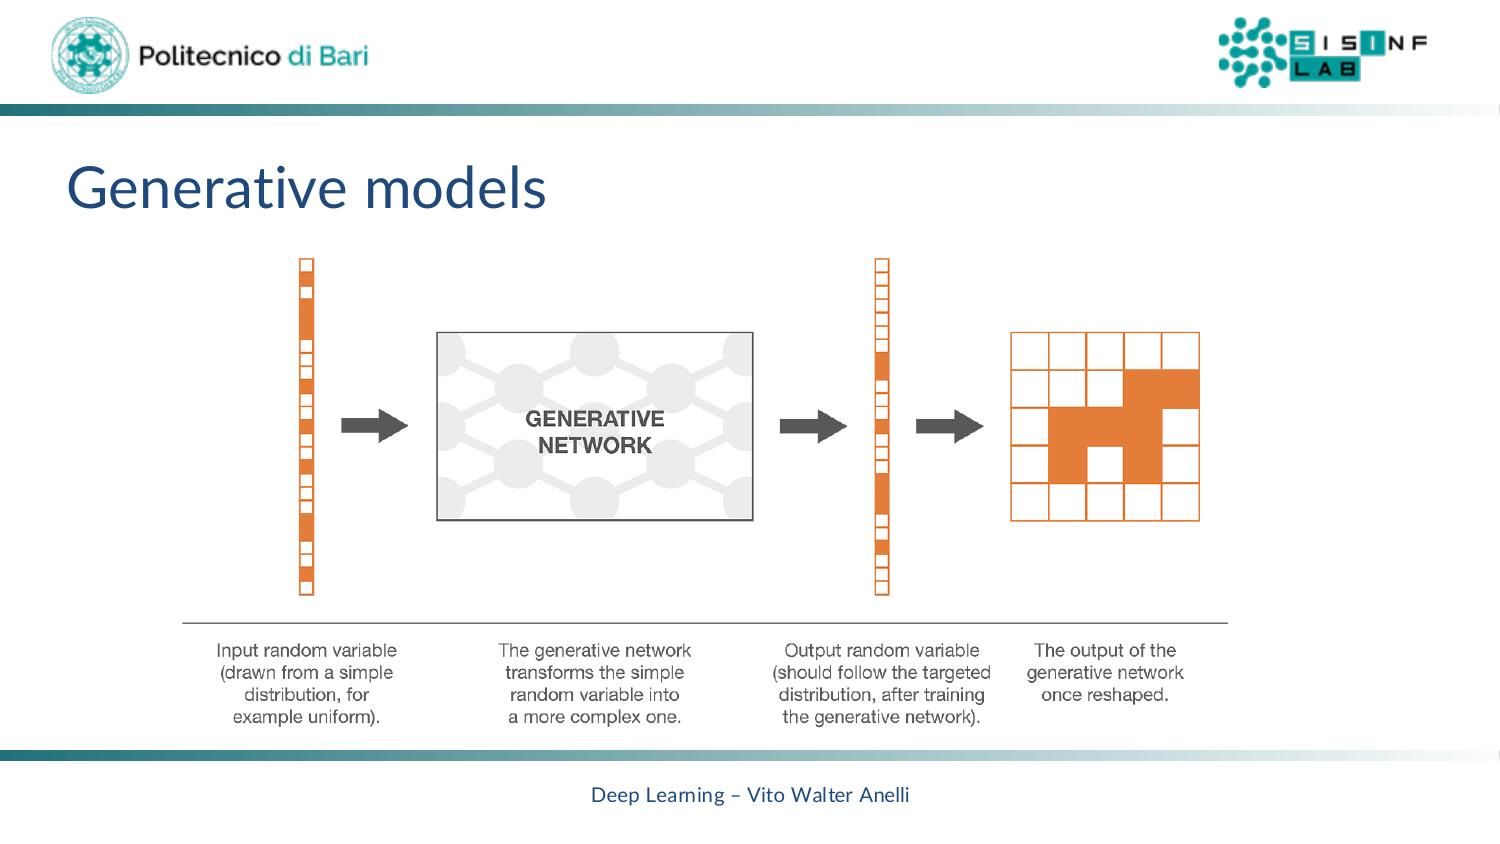
\includegraphics[width=0.82\linewidth]{figures/cf11_gan_generative_model.jpg}
  \caption{Schema di una rete generativa. Una variabile casuale campionata
           da una distribuzione semplice (uniforme) viene trasformata
           dalla rete in un vettore ad alta dimensionalità che, una volta
           ridimensionato a matrice, produce un'immagine sintetica. Dopo
           l'addestramento, la distribuzione dell'output deve coincidere
           con la distribuzione target.}
  \label{fig:gan_generative_model}
\end{figure}

\subsubsection{Addestramento Diretto}

L'approccio ``diretto'' consiste nel ripetere iterativamente i seguenti
passi:

\begin{enumerate}
  \item Campionare alcuni input uniformi $\mathbf{z}$.
  \item Propagarli attraverso la rete e raccogliere gli output generati
        $\mathbf{x}' = G(\mathbf{z})$.
  \item Confrontare la distribuzione generata con quella reale usando una
        metrica campionaria (es.\ la \emph{Maximum Mean Discrepancy},
        MMD).
  \item Eseguire un passo di discesa del gradiente per ridurre la
        distanza tra le due distribuzioni.
\end{enumerate}

\begin{figure}[H]
  \centering
  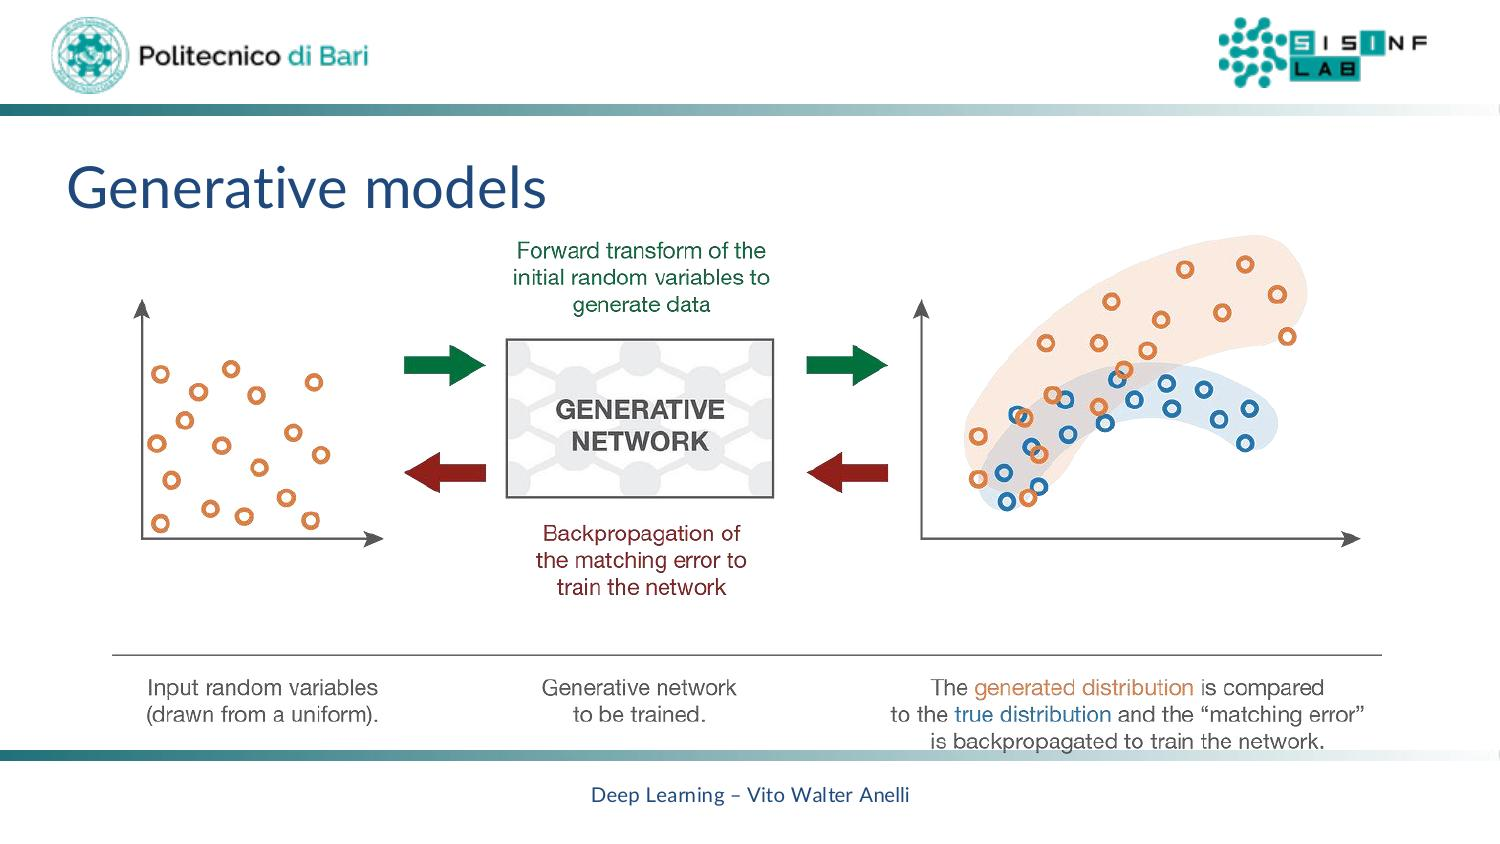
\includegraphics[width=0.82\linewidth]{figures/cf11_gan_training_loop.jpg}
  \caption{Schema dell'addestramento diretto di una rete generativa.
           La distribuzione generata (arancione) viene confrontata con
           quella reale (blu) e l'errore di corrispondenza viene
           retropropagato per aggiornare i pesi della rete.}
  \label{fig:gan_training_loop}
\end{figure}

La difficoltà principale di questo approccio è che il confronto diretto
tra distribuzioni di probabilità a partire da campioni è
computazionalmente costoso e spesso mal condizionato in alta dimensione.
Le GAN propongono una soluzione elegante a questo problema.

%------------------------------------------------------------
\section{Generative Adversarial Networks}
\label{sec:gan-core}

\subsection{L'Idea Fondamentale: Confronto Indiretto}
\label{subsec:gan-idea}

La brillante intuizione alla base delle GAN consiste nel rimpiazzare
il confronto diretto tra distribuzioni con uno \textbf{indiretto}, che
assume la forma di un task a valle (\emph{downstream task}) di
discriminazione tra campioni reali e campioni generati. L'addestramento
del generatore viene svolto rispetto a questo task in modo tale che la
distribuzione generata venga spinta progressivamente verso quella reale
\citep{bishop2024}.

Il task a valle è un \textbf{problema di classificazione binaria}: dato
un campione, determinare se esso proviene dalla distribuzione reale
(``vero'') o dal generatore (``falso''). Dal punto di vista del
generatore, si tratta di un task di \emph{non-discriminazione}: si
vuole che la classificazione fallisca il più possibile.

\subsection{Architettura GAN}
\label{subsec:gan-arch}

In un'architettura GAN sono presenti due reti:

\begin{description}
  \item[Generatore $G$] Rete neurale che modella una funzione di
        trasformazione. Riceve in input una variabile latente
        $\mathbf{z} \in \mathbb{R}^d$ campionata da una distribuzione
        semplice (tipicamente $\mathbf{z} \sim \mathcal{N}(\mathbf{0},
        \mathbf{I})$) e produce un campione sintetico
        $\mathbf{x}' = G(\mathbf{z})$.
        L'obiettivo, una volta addestrato, è che $\mathbf{x}'$ segua
        la distribuzione target.
  \item[Discriminatore $D$] Rete neurale che modella una funzione
        discriminativa. Riceve in input un punto $\mathbf{x}$ (vettore
        $N$-dimensionale) e restituisce la probabilità stimata che tale
        punto provenga dalla distribuzione reale:
        $D(\mathbf{x}) \in [0, 1]$.
\end{description}

Le due reti vengono addestrate \textbf{congiuntamente} con obiettivi
opposti:

\begin{itemize}
  \item Il generatore cerca di \emph{ingannare} il discriminatore, ossia
        è addestrato a \textbf{massimizzare} l'errore di classificazione
        (gradiente ascendente sull'errore rispetto ai parametri di $G$).
  \item Il discriminatore cerca di \emph{rilevare} i campioni falsi,
        ossia è addestrato a \textbf{minimizzare} l'errore di
        classificazione (discesa del gradiente rispetto ai parametri
        di $D$).
\end{itemize}

\begin{figure}[H]
  \centering
  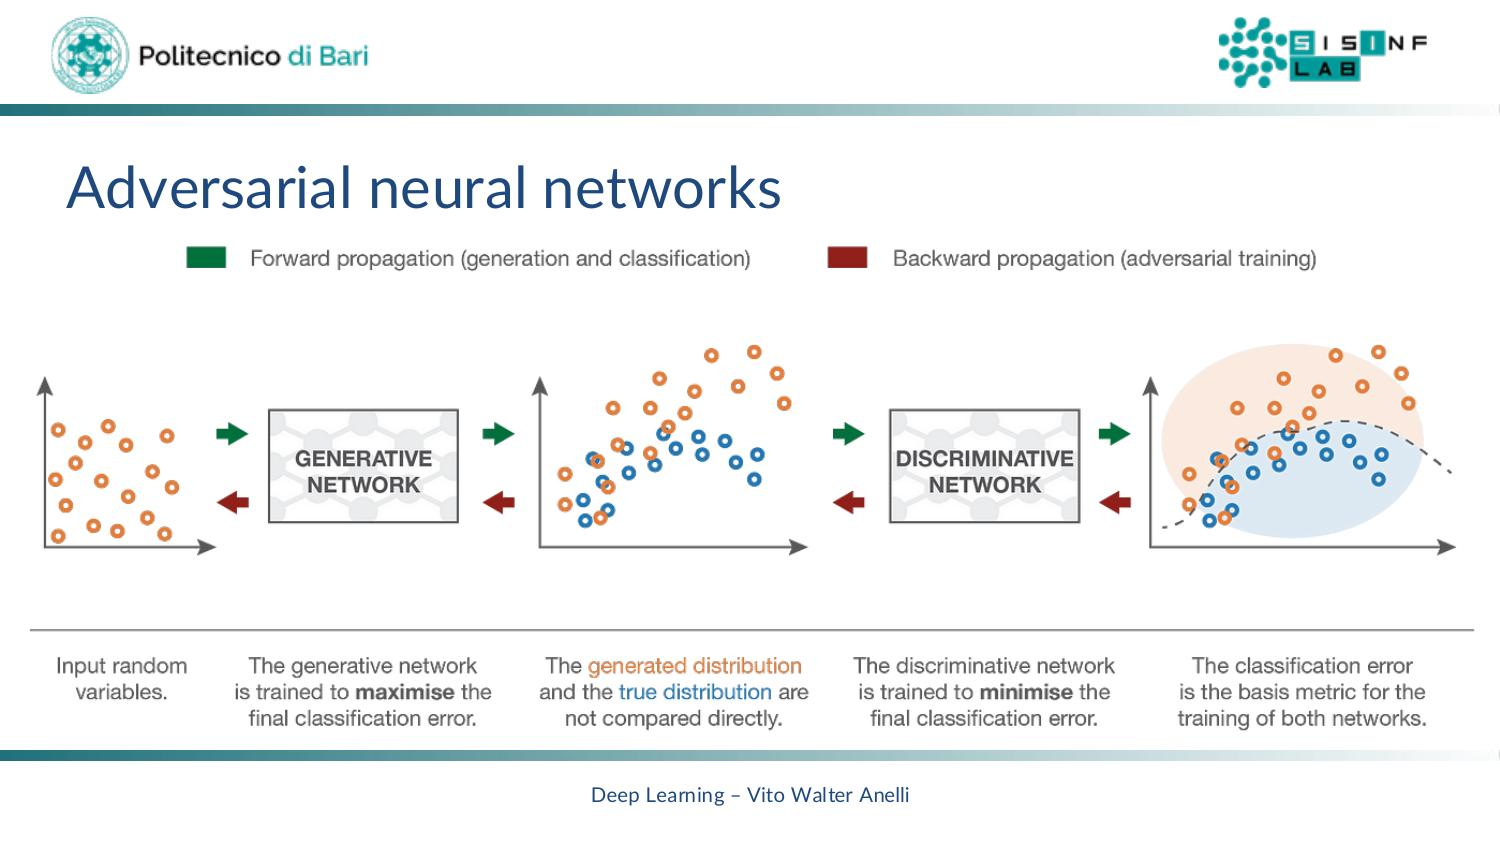
\includegraphics[width=0.95\linewidth]{figures/cf11_gan_adversarial_arch.jpg}
  \caption{Architettura adversariale. La rete generativa (sinistra)
           trasforma variabili casuali in campioni sintetici; la rete
           discriminativa (destra) riceve campioni reali e generati e
           tenta di classificarli correttamente. Le frecce rosse
           rappresentano la backpropagation avversariale: il generatore
           è addestrato a massimizzare l'errore di classificazione,
           il discriminatore a minimizzarlo.}
  \label{fig:gan_adversarial_arch}
\end{figure}

\subsection{Architettura Pratica}
\label{subsec:gan-practical-arch}

\begin{figure}[H]
  \centering
  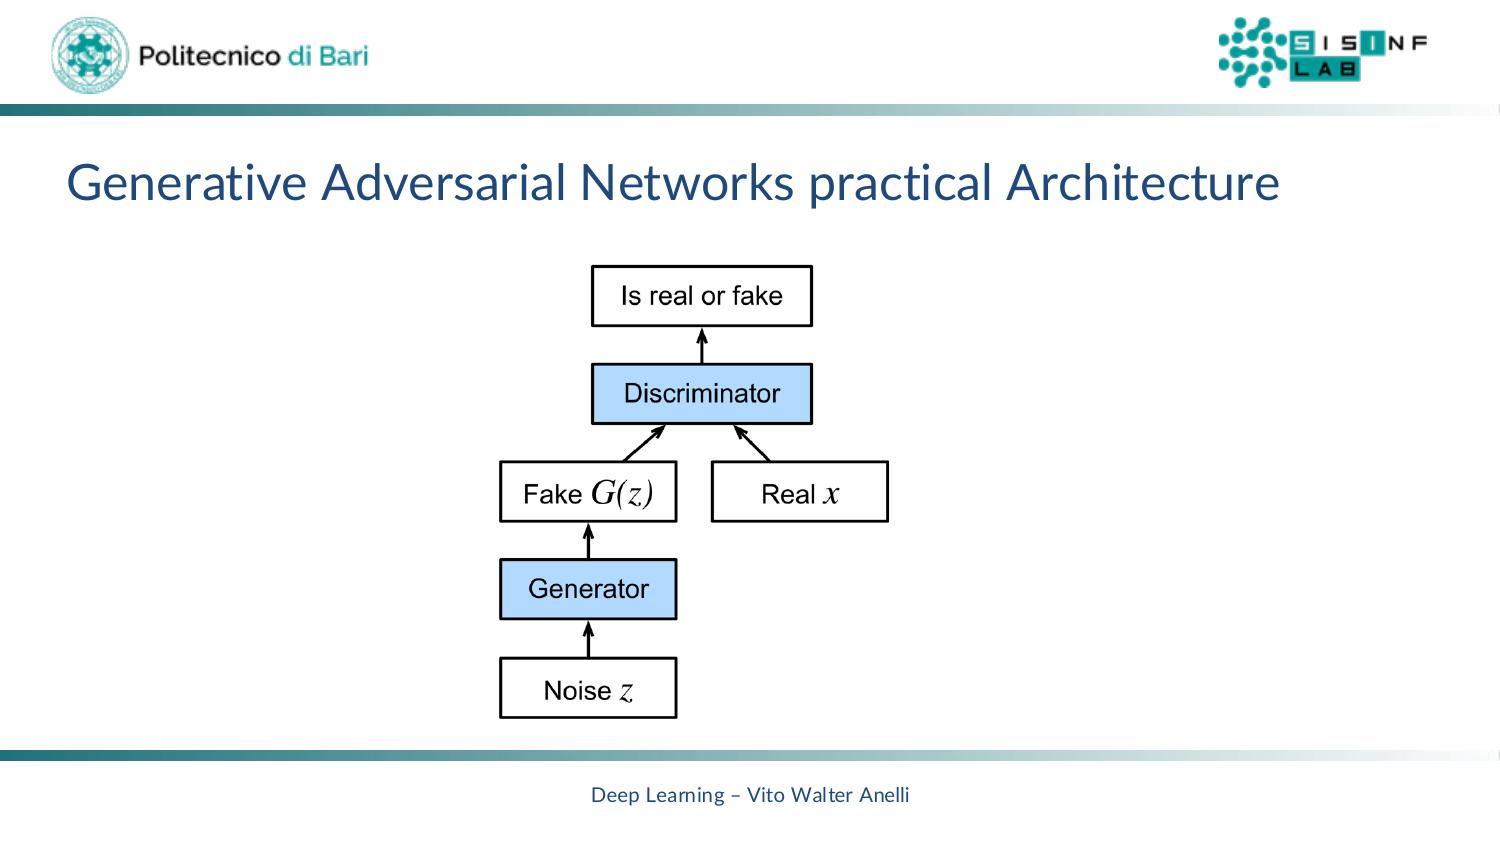
\includegraphics[width=0.60\linewidth]{figures/cf11_gan_practical_arch.jpg}
  \caption{Architettura GAN pratica. Il generatore riceve il rumore
           $\mathbf{z}$ e produce $G(\mathbf{z})$ (campione falso). Il
           discriminatore riceve sia i campioni reali $\mathbf{x}$ che
           quelli falsi $G(\mathbf{z})$ e produce una predizione scalare
           (\emph{reale} o \emph{falso}).}
  \label{fig:gan_practical_arch}
\end{figure}

%------------------------------------------------------------
\section{Formulazione Matematica}
\label{sec:gan-math}

\subsection{Loss del Discriminatore}
\label{subsec:gan-loss-disc}

Il discriminatore è un classificatore binario. L'output è una
probabilità scalare $D(\mathbf{x}) = 1/(1 + e^{-o})$, dove $o$ è
l'uscita pre-sigmoid (tipicamente uno strato completamente connesso con
dimensione nascosta 1). Le etichette sono $y = 1$ per i dati reali e
$y = 0$ per quelli generati. La loss del discriminatore è la
\textbf{cross-entropy binaria}:

\begin{equation}
  \mathcal{L}_D = \min_{D}
    \Bigl\{-y \log D(\mathbf{x}) - (1 - y)\log(1 - D(\mathbf{x}))\Bigr\}.
  \label{eq:gan-disc-loss}
\end{equation}

Espandendo sulle due classi separatamente:

\begin{align}
  \mathcal{L}_D &= \min_{D}
    \Bigl\{-\mathbb{E}_{x \sim p_{\text{data}}} \log D(\mathbf{x})
           -\mathbb{E}_{z \sim p_z} \log(1 - D(G(\mathbf{z})))\Bigr\}.
  \label{eq:gan-disc-loss-expanded}
\end{align}

\subsection{Loss del Generatore}
\label{subsec:gan-loss-gen}

Per un dato discriminatore $D$, il generatore $G$ viene aggiornato per
massimizzare la cross-entropy loss quando $y = 0$, ovvero:

\begin{equation}
  \max_{G}\bigl\{-(1-y)\log(1 - D(G(\mathbf{z})))\bigr\}
    = \max_{G}\bigl\{-\log(1 - D(G(\mathbf{z})))\bigr\}.
  \label{eq:gan-gen-loss-orig}
\end{equation}

Tuttavia, quando il generatore produce campioni di qualità
($D(G(\mathbf{z})) \approx 1$), la funzione
$-\log(1 - D(G(\mathbf{z})))$ tende a zero e i gradienti risultano
troppo piccoli per fare progressi efficaci. Si preferisce quindi
minimizzare la seguente loss equivalente (con i target etichettati come
se fossero reali, $y = 1$):

\begin{equation}
  \min_{G}\bigl\{\log(1 - D(G(\mathbf{z})))\bigr\}
    \approx \max_{G}\bigl\{-\log(D(G(\mathbf{z})))\bigr\}.
  \label{eq:gan-gen-loss-flip}
\end{equation}

Questa formulazione (\emph{non-saturating GAN loss}) ha gradienti
significativi anche nelle prime fasi dell'addestramento, quando il
discriminatore riesce facilmente a distinguere campioni reali da falsi.

\subsection{Obiettivo Minimax Complessivo}
\label{subsec:gan-minimax}

Unificando le due loss, $D$ e $G$ giocano un gioco minimax a due
giocatori con la seguente funzione obiettivo:

\begin{equation}
  \min_{D}\max_{G}
    \Bigl\{-\mathbb{E}_{x \sim p_{\text{data}}} \log D(\mathbf{x})
           -\mathbb{E}_{z \sim p_z} \log(1 - D(G(\mathbf{z})))\Bigr\}.
  \label{eq:gan-minimax}
\end{equation}

\begin{figure}[H]
  \centering
  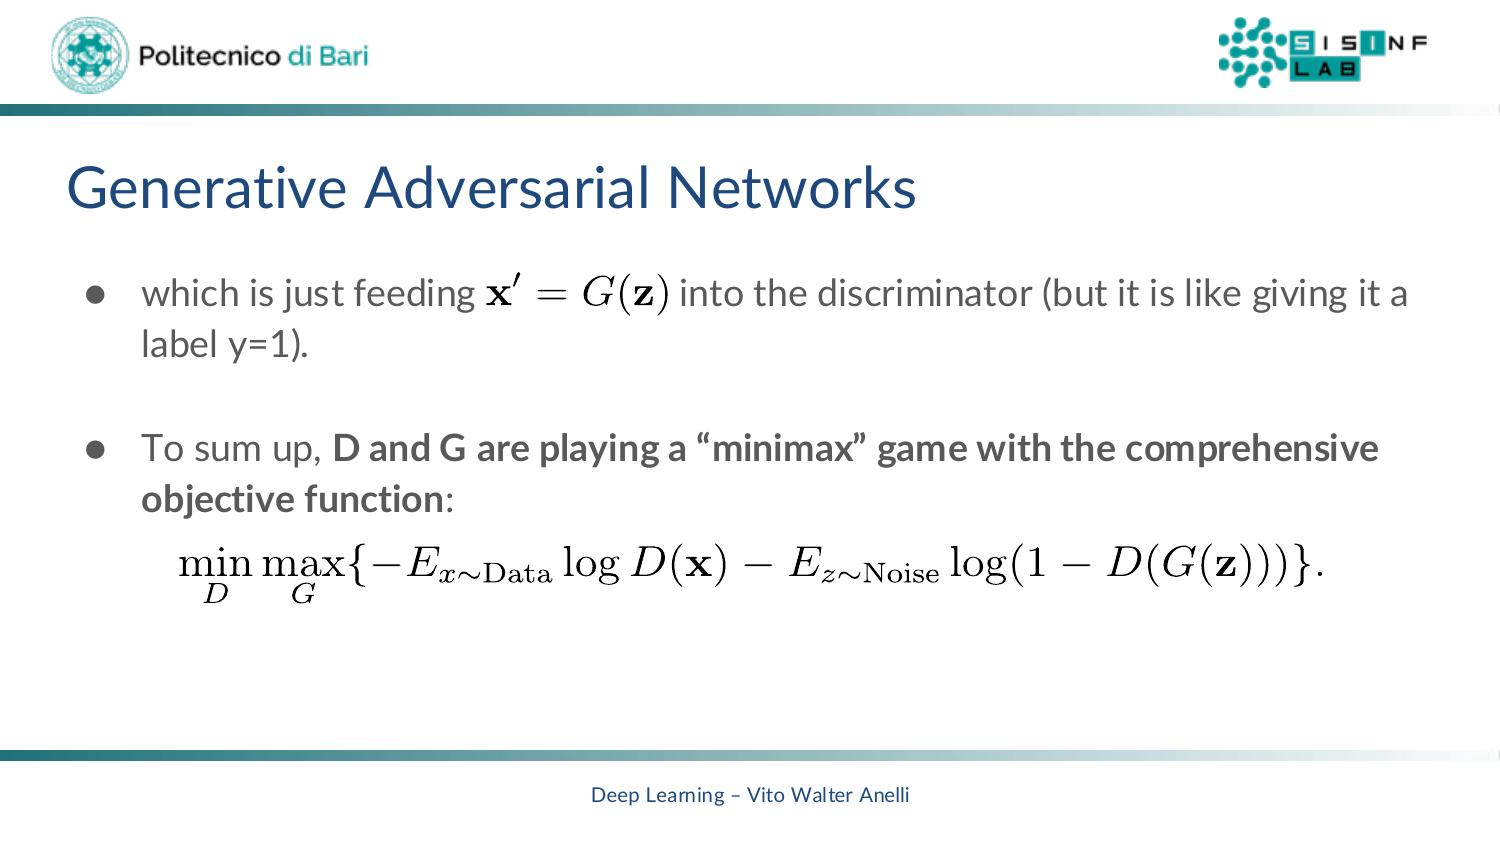
\includegraphics[width=0.82\linewidth]{figures/cf11_gan_minimax.jpg}
  \caption{Obiettivo minimax della GAN. Il discriminatore $D$ minimizza
           la cross-entropy binaria; il generatore $G$ la massimizza
           alimentando campioni falsi $G(\mathbf{z})$ nel discriminatore
           come se fossero reali ($y = 1$).}
  \label{fig:gan_minimax}
\end{figure}

\subsection{Interpretazione Game-Theoretic}
\label{subsec:gan-game-theory}

Dal punto di vista della teoria dei giochi, questa formulazione
corrisponde a un \textbf{gioco minimax a due giocatori}. Lo stato di
equilibrio (equilibrio di Nash) è raggiunto quando:

\begin{itemize}
  \item Il generatore produce campioni dalla distribuzione target esatta:
        $p_G = p_{\text{data}}$.
  \item Il discriminatore non riesce a fare meglio di una classificazione
        casuale: $D(\mathbf{x}) = 1/2$ per ogni punto $\mathbf{x}$.
\end{itemize}

Si può dimostrare che, a questo equilibrio, l'obiettivo minimax
equivale a minimizzare la \textbf{Jensen-Shannon Divergence} (JSD) tra
$p_{\text{data}}$ e $p_G$ \citep{bishop2024}:

\begin{equation}
  \mathcal{L}^* = -2\log 2
    + 2 \cdot \mathrm{JSD}(p_{\text{data}} \| p_G).
  \label{eq:gan-jsd}
\end{equation}

L'obiettivo è quindi minimizzare la JSD, che è zero se e solo se
$p_G = p_{\text{data}}$.

%------------------------------------------------------------
\section{Dinamica dell'Addestramento}
\label{sec:gan-training}

\subsection{Il Caso Ideale: Discriminatore Oracolo}
\label{subsec:gan-ideal-case}

Per comprendere la dinamica adversariale si consideri il caso
monodimensionale in cui la distribuzione target è una gaussiana
$\mathcal{N}(\mu, \sigma^2)$ e il generatore produce campioni da
un'altra gaussiana con parametri diversi.

Nell'approccio diretto, il generatore viene aggiornato
iterativamente correggendo la differenza misurata tra le due
distribuzioni fino a convergenza. Con un discriminatore oracolo (che
conosce esattamente le due distribuzioni), il gradiente fornito al
generatore è proporzionale alla differenza puntuale tra le densità.
Man mano che le due gaussiane si avvicinano, il discriminatore fatica
sempre di più a distinguerle, e all'equilibrio --- quando le
distribuzioni coincidono --- la sua accuratezza degrada a $50\%$.

\begin{figure}[H]
  \centering
  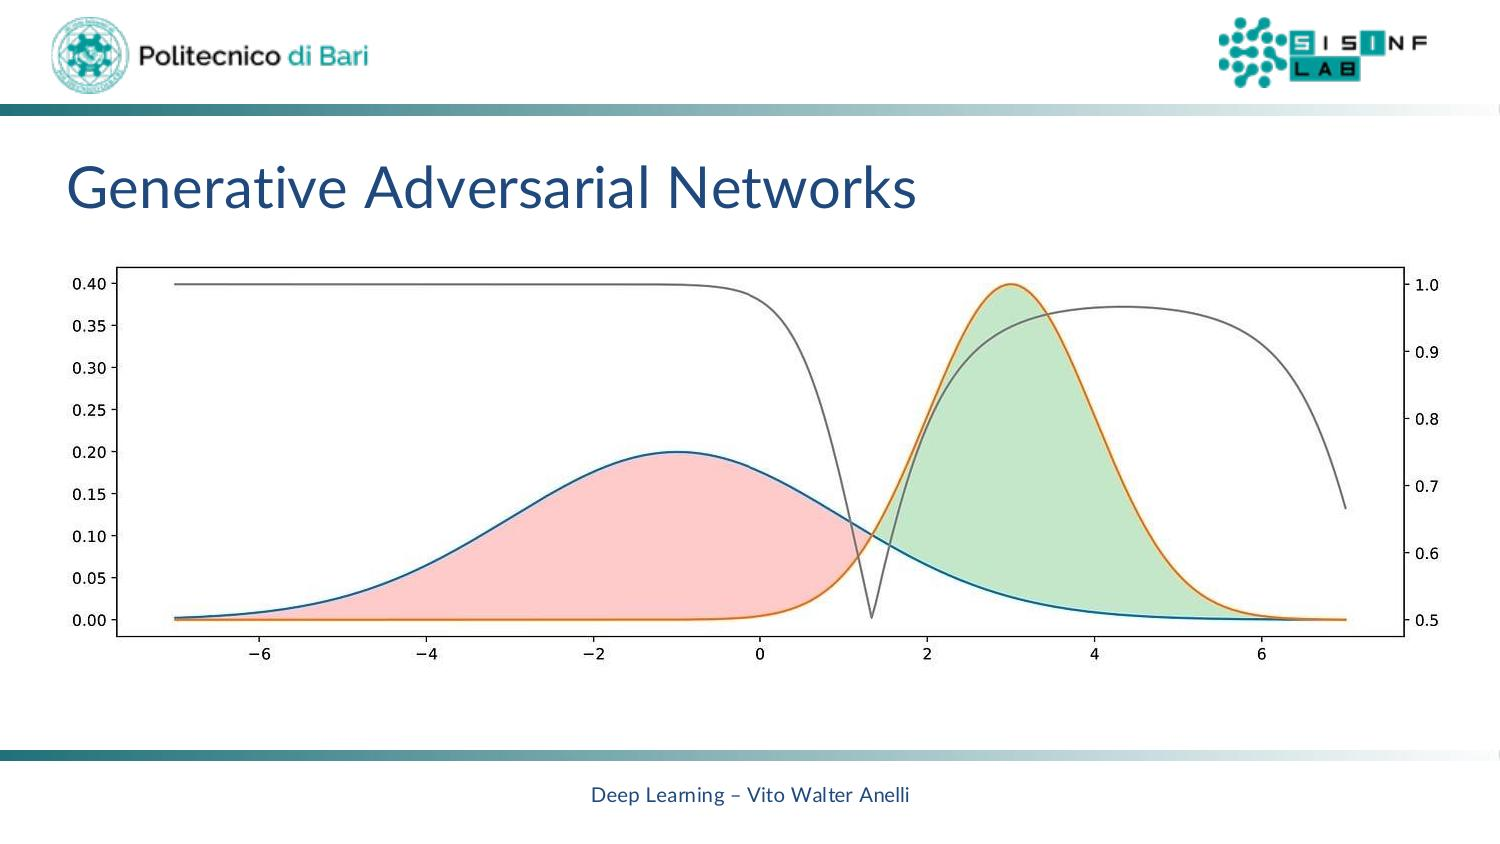
\includegraphics[width=0.82\linewidth]{figures/cf11_gan_discriminator_viz.jpg}
  \caption{Visualizzazione della dinamica discriminatore--generatore.
           In blu: distribuzione reale; in arancione: distribuzione
           generata. In grigio (asse destro): probabilità predetta dal
           discriminatore oracolo. L'area rossa indica le regioni in
           cui la distribuzione generata è in eccesso rispetto alla
           reale (da ridurre); l'area verde le regioni in difetto (da
           aumentare). Quanto più le due distribuzioni si sovrappongono,
           tanto più spesso il discriminatore commette errori.}
  \label{fig:gan_discriminator_viz}
\end{figure}

\subsection{L'Approssimazione Pratica: Reti Neurali}
\label{subsec:gan-approx}

Nella pratica, né il generatore né il discriminatore sono oracoli:
entrambi vengono approssimati con reti neurali e addestrati
congiuntamente. Ad ogni iterazione del ciclo di addestramento:

\begin{enumerate}
  \item I pesi della rete generativa vengono aggiornati in direzione di
        \textbf{ascesa del gradiente} rispetto all'errore di
        classificazione (i.e., $G$ cerca di aumentare l'errore).
  \item I pesi della rete discriminativa vengono aggiornati in direzione
        di \textbf{discesa del gradiente} rispetto allo stesso errore
        (i.e., $D$ cerca di ridurre l'errore).
\end{enumerate}

In questo modo entrambe le reti ``progrediscono'' rispetto ai propri
obiettivi, migliorandosi a vicenda: il discriminatore più capace spinge
il generatore a produrre campioni migliori; il generatore più convincente
costringe il discriminatore a diventare più selettivo. Questo meccanismo
di co-evoluzione dà il nome di \emph{adversarial training}.

\subsection{Procedura di Addestramento}
\label{subsec:gan-training-procedure}

L'algoritmo di addestramento alterna aggiornamenti del discriminatore e
del generatore. Nella formulazione originale \citep{bishop2024}:

\begin{enumerate}
  \item \textbf{Aggiornamento del Discriminatore} (k passi):
        \begin{enumerate}
          \item Campionare un mini-batch di dati reali
                $\{\mathbf{x}^{(i)}\}_{i=1}^{m}$ da $p_{\text{data}}$.
          \item Campionare un mini-batch di rumore latente
                $\{\mathbf{z}^{(i)}\}_{i=1}^{m}$ da $p_z$.
          \item Aggiornare $D$ con discesa del gradiente stocastica:
                \[
                  \nabla_{\theta_D} \frac{1}{m} \sum_{i=1}^{m}
                  \Bigl[\log D(\mathbf{x}^{(i)})
                       + \log\bigl(1 - D(G(\mathbf{z}^{(i)}))\bigr)\Bigr].
                \]
        \end{enumerate}
  \item \textbf{Aggiornamento del Generatore} (1 passo):
        \begin{enumerate}
          \item Campionare un mini-batch di rumore latente
                $\{\mathbf{z}^{(i)}\}_{i=1}^{m}$ da $p_z$.
          \item Aggiornare $G$ con ascesa del gradiente stocastica:
                \[
                  \nabla_{\theta_G} \frac{1}{m} \sum_{i=1}^{m}
                  \log\bigl(D(G(\mathbf{z}^{(i)}))\bigr).
                \]
        \end{enumerate}
\end{enumerate}

Nella pratica, il discriminatore viene tipicamente aggiornato più volte
per ogni aggiornamento del generatore ($k > 1$), in modo da mantenere
il discriminatore ``più forte'' del generatore e fornire un segnale di
gradiente più informativo.

%------------------------------------------------------------
\section{Problematiche nell'Addestramento delle GAN}
\label{sec:gan-issues}

Nonostante l'eleganza teorica, l'addestramento delle GAN presenta
diverse difficoltà pratiche note.

\subsection{Mode Collapse}
\label{subsec:mode-collapse}

Il \textbf{mode collapse} si verifica quando il generatore impara a
produrre solo un sottoinsieme limitato di modi della distribuzione
target, ignorando la varietà presente nei dati reali. In casi estremi,
$G$ converge a produrre sempre lo stesso campione (o pochi campioni
simili), perché questo inganna sistematicamente il discriminatore.
Dal punto di vista della JSD, il mode collapse corrisponde a una
situazione in cui $p_G$ ha supporto molto più piccolo di
$p_{\text{data}}$.

\subsection{Instabilità dell'Addestramento}
\label{subsec:training-instability}

L'equilibrio di Nash del gioco minimax è difficile da raggiungere con
la discesa del gradiente stocastica, perché i gradienti dei due
giocatori interferiscono reciprocamente. Fenomeni tipici sono:

\begin{itemize}
  \item \textbf{Oscillazioni}: generatore e discriminatore non
        convergono ma oscillano in modo ciclico.
  \item \textbf{Vanishing gradients}: se il discriminatore diventa
        troppo forte, $D(G(\mathbf{z})) \approx 0$ e il gradiente
        verso $G$ svanisce.
  \item \textbf{Exploding gradients}: in alcune configurazioni di
        architettura, i gradienti esplodono.
\end{itemize}

\subsection{Soluzioni Proposte}
\label{subsec:gan-solutions}

Diverse varianti architetturali e algoritmiche sono state proposte per
mitigare queste problematiche:

\begin{description}
  \item[Wasserstein GAN (WGAN)] Sostituisce la JSD con la
        \emph{Wasserstein distance} (distanza di Earth Mover), che
        fornisce gradienti più stabili anche quando le distribuzioni
        hanno supporti disgiunti. Richiede il clipping dei pesi del
        discriminatore (o il \emph{gradient penalty}) per soddisfare
        il vincolo di Lipschitz.
  \item[DCGAN] Utilizza convoluzioni nel generatore e nel
        discriminatore, con batch normalization e funzioni di
        attivazione specifiche (ReLU nel generatore, LeakyReLU nel
        discriminatore), migliorando la stabilità su dati visivi.
  \item[Conditional GAN (cGAN)] Condiziona sia il generatore che il
        discriminatore su un'etichetta di classe $y$, permettendo la
        generazione controllata di campioni di una categoria specifica.
  \item[Progressive GAN] Addestra generatore e discriminatore in modo
        progressivo, aumentando gradualmente la risoluzione delle
        immagini sintetizzate.
\end{description}

%------------------------------------------------------------
\section{Implementazione in PyTorch}
\label{sec:gan-pytorch}

Di seguito è riportata un'implementazione minimalista di una GAN per
dati monodimensionali, che illustra i concetti chiave dell'addestramento
adversariale.

\begin{lstlisting}[language=Python,
  caption={GAN minimale in PyTorch: generatore, discriminatore e ciclo
           di addestramento.},
  label={lst:gan-pytorch}]
import torch
import torch.nn as nn
import torch.optim as optim

# -- Architetture ------------------------------------------------------
class Generator(nn.Module):
    def __init__(self, d_z: int, d_out: int):
        super().__init__()
        self.net = nn.Sequential(
            nn.Linear(d_z, 128), nn.ReLU(),
            nn.Linear(128, 256), nn.ReLU(),
            nn.Linear(256, d_out),
        )

    def forward(self, z):
        return self.net(z)


class Discriminator(nn.Module):
    def __init__(self, d_in: int):
        super().__init__()
        self.net = nn.Sequential(
            nn.Linear(d_in, 256), nn.LeakyReLU(0.2),
            nn.Linear(256, 128), nn.LeakyReLU(0.2),
            nn.Linear(128, 1),   nn.Sigmoid(),
        )

    def forward(self, x):
        return self.net(x)


# -- Iperparametri -----------------------------------------------------
d_z, d_x = 16, 1
G = Generator(d_z, d_x)
D = Discriminator(d_x)
criterion = nn.BCELoss()
opt_G = optim.Adam(G.parameters(), lr=1e-4)
opt_D = optim.Adam(D.parameters(), lr=1e-4)

# -- Ciclo di addestramento --------------------------------------------
for step in range(10_000):
    batch = 64
    real = torch.randn(batch, d_x) * 0.5 + 2.0  # target: N(2, 0.25)
    z    = torch.randn(batch, d_z)
    fake = G(z).detach()                          # non backprop in G

    # -- Aggiornamento Discriminatore ----------------------------------
    loss_D = criterion(D(real), torch.ones(batch, 1)) \
           + criterion(D(fake), torch.zeros(batch, 1))
    opt_D.zero_grad(); loss_D.backward(); opt_D.step()

    # -- Aggiornamento Generatore --------------------------------------
    fake = G(torch.randn(batch, d_z))
    # non-saturating loss: massimizzare log D(G(z))
    loss_G = criterion(D(fake), torch.ones(batch, 1))
    opt_G.zero_grad(); loss_G.backward(); opt_G.step()
\end{lstlisting}

%------------------------------------------------------------
\section{Confronto tra Modelli Generativi}
\label{sec:gan-comparison}

\begin{table}[H]
  \centering
  \caption{Confronto tra i principali framework generativi.}
  \label{tab:gen-comparison}
  \small
  \begin{tabularx}{\linewidth}{l X X X}
    \toprule
    \textbf{Modello} & \textbf{Spazio latente}
      & \textbf{Qualità campioni} & \textbf{Criticità} \\
    \midrule
    VAE              & Distribuzione $\mathcal{N}(\boldsymbol{\mu}, \boldsymbol{\sigma}^2)$ & Media (campioni sfocati)    & Ottimizzazione ELBO \\
    GAN              & Vettore latente $\mathbf{z} \sim p_z$                               & Alta (campioni nitidi)      & Mode collapse, instabilità \\
    Normalizing Flow & Biiezione esatta                                                     & Alta (log-likelihood esatta)& Architettura vincolata \\
    Diffusion Model  & Processo di diffusione                                               & Molto alta (SOTA)           & Inferenza lenta \\
    \bottomrule
  \end{tabularx}
\end{table}

Le GAN eccellono nella \textbf{qualità visiva} dei campioni generati,
in particolare per immagini ad alta risoluzione, ma richiedono una
calibrazione attenta degli iperparametri e dell'architettura per evitare
mode collapse e instabilità. I modelli di diffusione, più recenti, hanno
in larga misura superato le GAN sulla qualità generativa al costo di
un'inferenza più lenta, ma le GAN rimangono rilevanti per applicazioni
in tempo reale e per la loro interpretazione game-theoretic
\citep{bishop2024}.

\paragraph{Considerazioni pratiche.}
\begin{enumerate}
  \item Per la \textbf{generazione di immagini ad alta risoluzione}
        preferire DCGAN o Progressive GAN con batch normalization.
  \item Per \textbf{stabilità di addestramento}: usare la Wasserstein
        loss con gradient penalty (WGAN-GP) invece della cross-entropy
        standard; il discriminatore non deve saturare prima che il
        generatore abbia avuto modo di aggiornarsi.
  \item Monitorare sia la loss del discriminatore che quella del
        generatore: se $\mathcal{L}_D \to 0$, il discriminatore ha
        preso troppo vantaggio e il segnale verso $G$ svanisce.
  \item La \textbf{non-saturating loss} (eq.~\ref{eq:gan-gen-loss-flip})
        fornisce gradienti più stabili rispetto alla formulazione
        minimax originale e deve essere preferita nella pratica.
  \item Il \textbf{mode collapse} può essere diagnosticato monitorando
        la varianza dei campioni generati su mini-batch successivi; se
        la varianza crolla, il generatore ha collassato su pochi modi.
\end{enumerate}
